\chapter{Bipartite graph}
    \section{Complete bipartite graph}
        Let's call $K_{m,n}$a complete bipartite graph
        \begin{figure}[h]%TODO
            \centering
            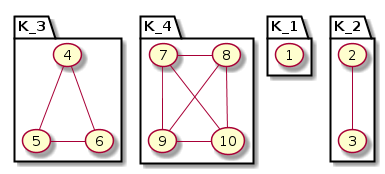
\includegraphics[scale=0.5]{ressources/images/CompleteGraphs.png}
            \caption{Every complete graph from $K_0$ to $K_4$}
            \label{Complete graph}
        \end{figure}
    \section{Euler tours}
        \subsection{Definition}
            A circuit is \textbf{Eulerian} if it contains every edge
        \subsection{Theorem}
            $G$ has a Eulerian circuit $\Leftrightarrow G\backslash$ (isolated vertices) is coonnected and every vertex has even degree
        \subsection{Proof}
            \begin{itemize}
                \item $\Rightarrow$: We may assume $G$ has no isolated vertices $\Rightarrow$ $C$ contains a walk from $v$ to $w$
                \item $\Leftarrow$: Induction on $|V(G)|+|E(G)|$\\
                    We may assume $G$ is connected (by removing isolated vertices)\\
                    We may assume $|V(G)|>1$\\
                    $G$ contains a cycle $C$ (Else, it would be a tree)\\
                    By the induction hyp, each non trivial component of $H$ has an Eulerian circuit
            \end{itemize}

